\documentclass[mstat,12pt]{unswthesis}

\usepackage{color}
\usepackage{fancyvrb}
\newcommand{\VerbBar}{|}
\newcommand{\VERB}{\Verb[commandchars=\\\{\}]}
\DefineVerbatimEnvironment{Highlighting}{Verbatim}{commandchars=\\\{\}}
% Add ',fontsize=\small' for more characters per line
\usepackage{framed}
\definecolor{shadecolor}{RGB}{248,248,248}
\newenvironment{Shaded}{\begin{snugshade}}{\end{snugshade}}
\newcommand{\AlertTok}[1]{\textcolor[rgb]{0.94,0.16,0.16}{#1}}
\newcommand{\AnnotationTok}[1]{\textcolor[rgb]{0.56,0.35,0.01}{\textbf{\textit{#1}}}}
\newcommand{\AttributeTok}[1]{\textcolor[rgb]{0.77,0.63,0.00}{#1}}
\newcommand{\BaseNTok}[1]{\textcolor[rgb]{0.00,0.00,0.81}{#1}}
\newcommand{\BuiltInTok}[1]{#1}
\newcommand{\CharTok}[1]{\textcolor[rgb]{0.31,0.60,0.02}{#1}}
\newcommand{\CommentTok}[1]{\textcolor[rgb]{0.56,0.35,0.01}{\textit{#1}}}
\newcommand{\CommentVarTok}[1]{\textcolor[rgb]{0.56,0.35,0.01}{\textbf{\textit{#1}}}}
\newcommand{\ConstantTok}[1]{\textcolor[rgb]{0.00,0.00,0.00}{#1}}
\newcommand{\ControlFlowTok}[1]{\textcolor[rgb]{0.13,0.29,0.53}{\textbf{#1}}}
\newcommand{\DataTypeTok}[1]{\textcolor[rgb]{0.13,0.29,0.53}{#1}}
\newcommand{\DecValTok}[1]{\textcolor[rgb]{0.00,0.00,0.81}{#1}}
\newcommand{\DocumentationTok}[1]{\textcolor[rgb]{0.56,0.35,0.01}{\textbf{\textit{#1}}}}
\newcommand{\ErrorTok}[1]{\textcolor[rgb]{0.64,0.00,0.00}{\textbf{#1}}}
\newcommand{\ExtensionTok}[1]{#1}
\newcommand{\FloatTok}[1]{\textcolor[rgb]{0.00,0.00,0.81}{#1}}
\newcommand{\FunctionTok}[1]{\textcolor[rgb]{0.00,0.00,0.00}{#1}}
\newcommand{\ImportTok}[1]{#1}
\newcommand{\InformationTok}[1]{\textcolor[rgb]{0.56,0.35,0.01}{\textbf{\textit{#1}}}}
\newcommand{\KeywordTok}[1]{\textcolor[rgb]{0.13,0.29,0.53}{\textbf{#1}}}
\newcommand{\NormalTok}[1]{#1}
\newcommand{\OperatorTok}[1]{\textcolor[rgb]{0.81,0.36,0.00}{\textbf{#1}}}
\newcommand{\OtherTok}[1]{\textcolor[rgb]{0.56,0.35,0.01}{#1}}
\newcommand{\PreprocessorTok}[1]{\textcolor[rgb]{0.56,0.35,0.01}{\textit{#1}}}
\newcommand{\RegionMarkerTok}[1]{#1}
\newcommand{\SpecialCharTok}[1]{\textcolor[rgb]{0.00,0.00,0.00}{#1}}
\newcommand{\SpecialStringTok}[1]{\textcolor[rgb]{0.31,0.60,0.02}{#1}}
\newcommand{\StringTok}[1]{\textcolor[rgb]{0.31,0.60,0.02}{#1}}
\newcommand{\VariableTok}[1]{\textcolor[rgb]{0.00,0.00,0.00}{#1}}
\newcommand{\VerbatimStringTok}[1]{\textcolor[rgb]{0.31,0.60,0.02}{#1}}
\newcommand{\WarningTok}[1]{\textcolor[rgb]{0.56,0.35,0.01}{\textbf{\textit{#1}}}}


%%%%%%%%%%%%%%%%%%%%%%%%%%%%%%%%%%%%%%%%%%%%%%%%%%%%%%%%%%%%%%%%%%
% 
% OK...Now we get to some actual input.  The first part sets up
% the title etc that will appear on the front page
%
%%%%%%%%%%%%%%%%%%%%%%%%%%%%%%%%%%%%%%%%%%%%%%%%%%%%%%%%%%%%%%%%%

\title{Projet réalisé par l'équipe Groupe 6\\[0.5cm]Rapport de groupe en
Sciences des Données 2 + Bases de données}

\authornameonly{LOUATI Chamss-Eddine, NDIAYE Ibrahima , EL OUALYDY
Mohamed Amine, SARTORI Adrien }

\author{\Authornameonly}

\copyrightfalse
\figurespagefalse
\tablespagefalse

%%%%%%%%%%%%%%%%%%%%%%%%%%%%%%%%%%%%%%%%%%%%%%%%%%%%%%%%%%%%%%%%%
%
%  And now the document begins
%  The \beforepreface and \afterpreface commands puts the
%  contents page etc in
%
%%%%%%%%%%%%%%%%%%%%%%%%%%%%%%%%%%%%%%%%%%%%%%%%%%%%%%%%%%%%%%%%%%


%%%%%%%%%%%%%%%%%%%%%%%%%%%%%%%%%%%%%%%%%%%%%%%%%%%%%%%%%%%%%%%%%%%%%%%
%
%  A small sample UNSW Coursework Masters thesis file.
%  Any questions to Ian Doust i.doust@unsw.edu.au and/or Gery Geenens ggeenens@unsw.edu.au
%
%%%%%%%%%%%%%%%%%%%%%%%%%%%%%%%%%%%%%%%%%%%%%%%%%%%%%%%%%%%%%%%%%%%%%%%
%
%  The first part pulls in a UNSW Thesis class file.  This one is
%  slightly nonstandard and has been set up to do a couple of
%  things automatically
%
 
%%%%%%%%%%%%%%%%%
%% Precisely one of the next four lines should be uncommented.
%% Choose the one which matches your degree, uncomment it, and comment out the other two!
%\documentclass[mfin,12pt]{unswthesis}    %%  For Master of Financial Mathematics 
%\documentclass[mmath,12pt]{unswthesis}   %%  For Master of Mathematics
%\documentclass[mstat,12pt]{unswthesis}  %%  For Master of Statistics
%%%%%%%%%%%%%%%%%



\linespread{1}
\usepackage{amsfonts}
\usepackage{amssymb}
\usepackage{amsthm}
\usepackage{latexsym,amsmath}
\usepackage{graphicx}
\usepackage{afterpage}
\usepackage[colorlinks]{hyperref}
 \hypersetup{
     colorlinks=true,
     linkcolor=blue,
     filecolor=blue,
     citecolor= black,      
     urlcolor=cyan,
     }
\usepackage{textcomp}
\usepackage{longtable}
\usepackage{booktabs}
\usepackage{float}
\let\origfigure\figure
\let\endorigfigure\endfigure
\renewenvironment{figure}[1][2] {
    \expandafter\origfigure\expandafter[H]
} {
    \endorigfigure
}
\usepackage[T1]{fontenc}
\usepackage{ragged2e}
\def\tightlist{}

%%%%%%%%%%%%%%%%%%%%%%%%%%%%%%%%%%%%%%%%%%%%%%%%%%%%%%%%%%%%%%%%%
%
%  The following are some simple LaTeX macros to give some
%  commonly used letters in funny fonts. You may need more or less of
%  these
%
\newcommand{\R}{\mathbb{R}}
\newcommand{\Q}{\mathbb{Q}}
\newcommand{\C}{\mathbb{C}}
\newcommand{\N}{\mathbb{N}}
\newcommand{\F}{\mathbb{F}}
\newcommand{\PP}{\mathbb{P}}
\newcommand{\T}{\mathbb{T}}
\newcommand{\Z}{\mathbb{Z}}
\newcommand{\B}{\mathfrak{B}}
\newcommand{\BB}{\mathcal{B}}
\newcommand{\M}{\mathfrak{M}}
\newcommand{\X}{\mathfrak{X}}
\newcommand{\Y}{\mathfrak{Y}}
\newcommand{\CC}{\mathcal{C}}
\newcommand{\E}{\mathbb{E}}
\newcommand{\cP}{\mathcal{P}}
\newcommand{\cS}{\mathcal{S}}
\newcommand{\A}{\mathcal{A}}
\newcommand{\ZZ}{\mathcal{Z}}
%%%%%%%%%%%%%%%%%%%%%%%%%%%%%%%%%%%%%%%%%%%%%%%%%%%%%%%%%%%%%%%%%%%%%
%
% The following are much more esoteric commands that I have left in
% so that this file still processes. Use or delete as you see fit
%
\newcommand{\bv}[1]{\mbox{BV($#1$)}}
\newcommand{\comb}[2]{\left(\!\!\!\begin{array}{c}#1\\#2\end{array}\!\!\!\right)
}
\newcommand{\Lat}{{\rm Lat}}
\newcommand{\var}{\mathop{\rm var}}
\newcommand{\Pt}{{\mathcal P}}
\def\tr(#1){{\rm trace}(#1)}
\def\Exp(#1){{\mathbb E}(#1)}
\def\Exps(#1){{\mathbb E}\sparen(#1)}
\newcommand{\floor}[1]{\left\lfloor #1 \right\rfloor}
\newcommand{\ceil}[1]{\left\lceil #1 \right\rceil}
\newcommand{\hatt}[1]{\widehat #1}
\newcommand{\modeq}[3]{#1 \equiv #2 \,(\text{mod}\, #3)}
\newcommand{\rmod}{\,\mathrm{mod}\,}
\newcommand{\p}{\hphantom{+}}
\newcommand{\vect}[1]{\mbox{\boldmath $ #1 $}}
\newcommand{\reff}[2]{\ref{#1}.\ref{#2}}
\newcommand{\psum}[2]{\sum_{#1}^{#2}\!\!\!'\,\,}
\newcommand{\bin}[2]{\left( \begin{array}{@{}c@{}}
				#1 \\ #2
			\end{array}\right)	}
%
%  Macros - some of these are in plain TeX (gasp!)
%
\newcommand{\be}{($\beta$)}
\newcommand{\eqp}{\mathrel{{=}_p}}
\newcommand{\ltp}{\mathrel{{\prec}_p}}
\newcommand{\lep}{\mathrel{{\preceq}_p}}
\def\brack#1{\left \{ #1 \right \}}
\def\bul{$\bullet$\ }
\def\cl{{\rm cl}}
\let\del=\partial
\def\enditem{\par\smallskip\noindent}
\def\implies{\Rightarrow}
\def\inpr#1,#2{\t \hbox{\langle #1 , #2 \rangle} \t}
\def\ip<#1,#2>{\langle #1,#2 \rangle}
\def\lp{\ell^p}
\def\maxb#1{\max \brack{#1}}
\def\minb#1{\min \brack{#1}}
\def\mod#1{\left \vert #1 \right \vert}
\def\norm#1{\left \Vert #1 \right \Vert}
\def\paren(#1){\left( #1 \right)}
\def\qed{\hfill \hbox{$\Box$} \smallskip}
\def\sbrack#1{\Bigl \{ #1 \Bigr \} }
\def\ssbrack#1{ \{ #1 \} }
\def\smod#1{\Bigl \vert #1 \Bigr \vert}
\def\smmod#1{\bigl \vert #1 \bigr \vert}
\def\ssmod#1{\vert #1 \vert}
\def\sspmod#1{\vert\, #1 \, \vert}
\def\snorm#1{\Bigl \Vert #1 \Bigr \Vert}
\def\ssnorm#1{\Vert #1 \Vert}
\def\sparen(#1){\Bigl ( #1 \Bigr )}

\newcommand\blankpage{%
    \null
    \thispagestyle{empty}%
    \addtocounter{page}{-1}%
    \newpage}

%%%%%%%%%%%%%%%%%%%%%%%%%%%%%%%
%
% These environments allow you to get nice numbered headings
%  for your Theorems, Definitions etc.  
%
%  Environments
%
%%%%%%%%%%%%%%%%%%%%%%%%%%%%%%%

\newtheorem{theorem}{Theorem}[section]
\newtheorem{lemma}[theorem]{Lemma}
\newtheorem{proposition}[theorem]{Proposition}
\newtheorem{corollary}[theorem]{Corollary}
\newtheorem{conjecture}[theorem]{Conjecture}
\newtheorem{definition}[theorem]{Definition}
\newtheorem{example}[theorem]{Example}
\newtheorem{remark}[theorem]{Remark}
\newtheorem{question}[theorem]{Question}
\newtheorem{notation}[theorem]{Notation}
\numberwithin{equation}{section}

%%%%%%%%%%%%%%%%%%%%%%%%%%%%%%%%%%%%%%%%%%%%%%%%%%%%%%%%%%%%%%%%%%
%
%  If you've got some funny special words that LaTeX might not
% hyphenate properly, you can give it a helping hand:
%

\hyphenation{Mar-cin-kie-wicz Rade-macher}


\newlength{\cslhangindent}
\setlength{\cslhangindent}{1.5em}
\newlength{\csllabelwidth}
\setlength{\csllabelwidth}{3em}
\newenvironment{CSLReferences}[2] % #1 hanging-ident, #2 entry spacing
 {% don't indent paragraphs
  \setlength{\parindent}{0pt}
  % turn on hanging indent if param 1 is 1
  \ifodd #1 \everypar{\setlength{\hangindent}{\cslhangindent}}\ignorespaces\fi
  % set entry spacing
  \ifnum #2 > 0
  \setlength{\parskip}{#2\baselineskip}
  \fi
 }%
 {}
\usepackage{calc} % for \widthof, \maxof
\newcommand{\CSLBlock}[1]{#1\hfill\break}
\newcommand{\CSLLeftMargin}[1]{\parbox[t]{\maxof{\widthof{#1}}{\csllabelwidth}}{#1}}
\newcommand{\CSLRightInline}[1]{\parbox[t]{\linewidth}{#1}}
\newcommand{\CSLIndent}[1]{\hspace{\cslhangindent}#1}






\renewcommand{\contentsname}{Table des matières}

\renewcommand{\chaptername}{Chapitre}



\begin{document}

\beforepreface

%\afterpage{\blankpage}

% plagiarism

\prefacesection{Déclaration de non plagiat}

\vskip 2pc \noindent Nous déclarons que ce rapport est le fruit de notre seul travail, à part lorsque cela est indiqué  explicitement. 

\vskip 2pc  \noindent Nous acceptons que la personne évaluant ce rapport puisse, pour les besoins de cette évaluation:
\begin{itemize}
\item la reproduire et en fournir une copie à un autre membre de l'université; et/ou,
\item en communiquer une copie à un service en ligne de détection de plagiat (qui pourra en retenir une copie pour les besoins d'évaluation future).
\end{itemize}

\vskip 2pc \noindent Nous certifions que nous avons lu et compris les règles ci-dessus.\vspace{24pt}

\vskip 2pc \noindent En signant cette déclaration, nous acceptons ce qui précède.
\vskip 2pc \noindent
Signature: \rule{7cm}{0.25pt} \hfill Date: \rule{4cm}{0.25pt} \\[1cm]
Signature: \rule{7cm}{0.25pt} \hfill Date: \rule{4cm}{0.25pt} \\[1cm]
Signature: \rule{7cm}{0.25pt} \hfill Date: \rule{4cm}{0.25pt} \\[1cm]
Signature: \rule{7cm}{0.25pt} \hfill Date: \rule{4cm}{0.25pt} \\[1cm]
\vskip 1pc

%\afterpage{\blankpage}

% Acknowledgements are optional


\prefacesection{Remerciements}

{\bigskip}Nos plus sincères remerciements vont à notre encadrant
pédagogique pour les conseils avisés sur notre travail.\\[1cm] 

{\bigskip\bigskip\bigskip\noindent} 03/04/2023.

%\afterpage{\blankpage}

% Abstract

\prefacesection{Résumé}

Ce projet consiste à étudier des bases de données pour déterminer les
secteurs qui enregistrent le plus gros chiffre d'affaire au cours des
trois dernières années (2020, 2021, 2022), en particulier dans quelle
région. Nous avons importé nos données dans une base de données SQL,
puis effectué des analyses statistiques à l'aide de requêtes SQL et de
R. Nous avons utilisé R pour effectuer une analyse exploratoire de nos
données et identifier les secteurs d'activité les plus performants. Nous
avons ensuite créé des visualisations telles que des diagrammes en
barre, des nuages de points et des cartes pour mieux illustrer les
tendances économiques en France. Nos résultats peuvent aider les
investisseurs à mieux comprendre les tendances économiques en France et
à prendre des décisions d'investissement plus éclairées pour maximiser
leur rentabilité. .

\par

\bigskip

%\afterpage{\blankpage}


\afterpreface





%%%%%%%%%%%%%%%%%%%%%%%%%%%%%%%%%%%%%%%%%%%%%%%%%%%%%%%%%%%%%%%%%%
%
% Now we can start on the first chapter
% Within chapters we have sections, subsections and so forth
%
%%%%%%%%%%%%%%%%%%%%%%%%%%%%%%%%%%%%%%%%%%%%%%%%%%%%%%%%%%%%%%%%%%



%%%%%%%%%%%%%%%%%%%%%%%%%%%%%%%%%%%%%

%\afterpage{\blankpage}


\hypertarget{introduction}{%
\chapter{Introduction}\label{introduction}}

\hypertarget{contexualisation}{%
\section{Contexualisation}\label{contexualisation}}

En France, les secteurs qui enregistrent les plus gros chiffres
d'affaires ont une importance particulière en raison de leur
contribution significative à l'économie du pays. Connaître les secteurs
les plus performants peut aider les entreprises à mieux cibler leurs
investissements et à maximiser leur rentabilité. Les gouvernements
régionaux peuvent également utiliser ces informations pour développer
des politiques économiques qui favorisent les secteurs les plus
performants et stimulent la croissance économique régionale. Les trois
secteurs économiques principaux sont: \medskip

\begin{itemize}
  \item le secteur primaire : collecte et l'exploitation des ressources naturelles (matériaux, énergie, et certains aliments);
  \item le secteur secondaire : industries de transformation des matières premières;
  \item le secteur tertiaire : les industries du service;
  \end{itemize}

\medskip

Le but de ce projet sera de voir:

\bigskip

\centering

\textbf{Quels sont les secteurs d'activités qui enregistrent les plus
gros chiffres d'affaires et dans quelle région au cours de ces trois
dernières années(2020,2021,2022) ? }

\justifying

\bigskip

Pour ce faire, nous étudierons les chiffres d'affaires des entreprises
aisni que leurs localisations.

Les données utilisées seront celles trouvées sur le site :

\url{https://www.data.gouv.fr/fr/datasets/chiffres-cles-2022/}

\medskip

La question des secteurs d' activities qui enregistrent les plus gros
chiffres d'affaires revêt d'une grande importance pour un large éventail
d'acteurs économiques, notamment les investisseurs, les entreprises, les
gouvernements, les régulateurs et les consommateurs. Ainsi, l'actualité
de cette question est constante car les secteurs qui enregistrent les
plus gros chiffres d'affaires évoluent régulièrement en fonction des
changements économiques, technologiques et sociaux. Par conséquent,les
éléments de réponse à cette question pourront être utilisés pour des
actions variées.

\medskip

\hypertarget{base-de-donnuxe9es}{%
\chapter{Base de données}\label{base-de-donnuxe9es}}

\hypertarget{descriptif-des-tables}{%
\section{Descriptif des tables}\label{descriptif-des-tables}}

Notre base de données a été créée à partir d'un fichier appelé
``Chiffres clés 2022'' disponible sur le site web gouvernemental
français
``Data.gouv.fr''(\url{https://www.data.gouv.fr/fr/datasets/chiffres-cles-2022/}).
Le fichier initial contenait 167 885 lignes et 42 colonnes. Après
analyse et traitement des données, on a choisi de retenir trois tables
principales pour notre étude.

\begin{itemize}
\tightlist
\item
  \textbf{Table\_Activite}(5 colonnes, 443 lignes): Cette table a été
  créée pour mettre en évidence chaque secteur d'activité dans lequel
  l'entreprise appartient. On l'a réalisé en regroupant tous les
  secteurs d'activité pour faire la somme de leur chiffre d'affaire par
  année. Ce qui fait que dans cette table il n'y a pas de redondances au
  niveau de nos secteurs d'activité et que et pour chaque secteur on a
  le total de son chiffre d'affaire par années. Ainsi, elle est
  composée:

  \begin{itemize}
  \tightlist
  \item
    code d'activité(qui est de type \textbf{varchar} qui signifie
    caractère variable en francais),
  \item
    secteur d'activite(\textbf{varchar}),
  \item
    total chiffre d'affaire 2022(\textbf{bigint}, qui signifie gros
    entier en francais),
  \item
    total chiffre d'affaire 2021(\textbf{bigint}),
  \item
    total chiffre d'affaire 2020(\textbf{bigint})
  \end{itemize}
\item
  \textbf{Table\_Entreprise}(3.264 lignes,11 colonnes) : C'est notre
  table principale, où il y a le plus de colonnes et c'est la table où
  l'on retrouve toutes les caractéristiques de chaque entreprise:

  \begin{itemize}
  \tightlist
  \item
    identifiant de l'entreprise(\textbf{int}, qui signifie entier en
    francais),
  \item
    nom de l'entreprise(\textbf{varchar}),
  \item
    SIREN(\textbf{int}),
  \item
    code\_activite(\textbf{int}):clé étrangére référençant
    table\_activite,
  \item
    région (\textbf{varchar}), clé étrangére référençant table\_region,
  \item
    chiffre d'affaire 2022(\textbf{bigint}),
  \item
    chiffre d'affaire 2021(\textbf{bigint}),
  \item
    chiffre d'affaire 2020(\textbf{bigint}),
  \item
    effectif 2022(\textbf{int}),
  \item
    effectif 2021(\textbf{int}),
  \item
    effectif 2022(\textbf{int})
  \end{itemize}
\item
  \textbf{Table\_Region}(17 lignes, 4 colonnes): Ici aussi, on a realisé
  presque le même calcul pour les secteurs d'activités, on a regroupé
  toutes les régions de toutes les entreprises, et on a effectué la
  somme de leur chiffre d'affaire pour chaque année. Voici nos colonnes:

  \begin{itemize}
  \tightlist
  \item
    nom de la region(\textbf{varchar})
  \item
    total chiffre d'affaire 2022(\textbf{bigint})
  \item
    total chiffre d'affaire 2021(\textbf{bigint})
  \item
    total chiffre d'affaire 2022(\textbf{bigint})
  \end{itemize}
\end{itemize}

En résumé, notre base de données a été construite à partir d'un fichier
de données public, elle contient trois tables principales regroupant les
chiffres d'affaires et les caractéristiques des entreprises étudiées, et
elle est destinée à répondre à notre problématique de recherche des
secteurs d'activités les plus performants en termes de chiffres
d'affaires et de localisation.

\hypertarget{moduxe8les-mcd-et-mod}{%
\section{Modèles MCD et MOD}\label{moduxe8les-mcd-et-mod}}

\begin{itemize}
\tightlist
\item
  MCD :
\end{itemize}

\begin{figure}
\hypertarget{uml}{%
\centering
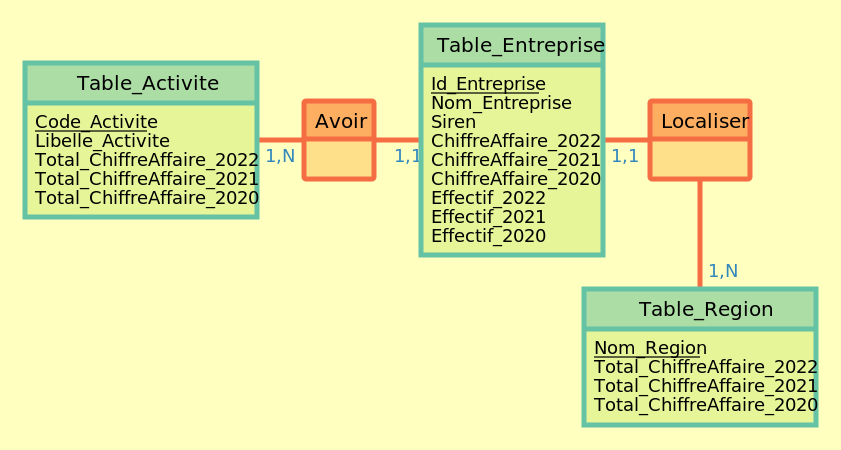
\includegraphics[width=14cm,height=10cm]{MCD.png}
\caption{MCD.}\label{uml}
}
\end{figure}

\begin{itemize}
\tightlist
\item
  MOD:
\end{itemize}

\includegraphics[width=14cm,height=10cm]{MoD.png} \bigskip

\textbf{Legende:} Dans l'explication de notre MOD le signe \textbf{\#}
représente les \textbf{clés étrangéres} et les mots soulignés sont les
\textbf{clés primaires}.

\begin{figure}
\hypertarget{uml}{%
\centering
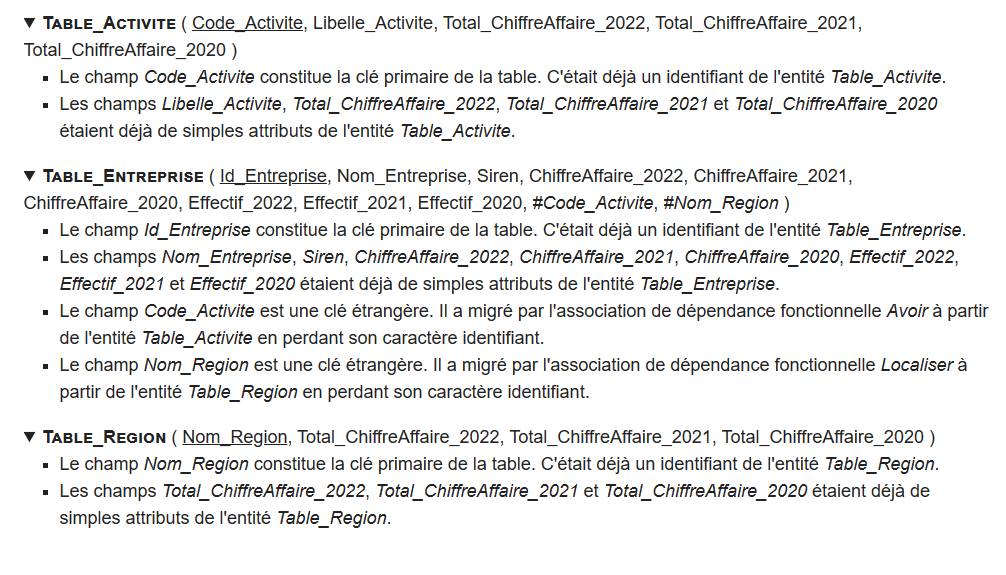
\includegraphics[width=14cm,height=10cm]{Explain_MOD.png}
\caption{Explication du MOD.}\label{uml}
}
\end{figure}

\bigskip

\hypertarget{import-des-donnuxe9es}{%
\section{Import des données}\label{import-des-donnuxe9es}}

\begin{itemize}
\item
  Le nettoyage des données a été réalisé sur Excel et Python(avec
  Pandas). Dans le fichier Chiffre clé 2022. Nous avons supprimé toutes
  les lignes comportants des valeurs manquantes. Pareillement, on a
  rectifié la forme d'écriture en UTF-8 pour rendre lisible nos données
  textuelles.
\item
  Nous avons aussi filtré le fichier chiffre clé afin d'avoir nos trois
  tables. Ainsi, on a pu tirer la table Region en regroupant les regions
  de toutes les entreprises en faisant la somme de leur chiffre
  d'affaires pour chaque année avec l'aide de la bibliothéque pandas,
  puis on a effectué la même tâche pour avoir la table Activité.
\end{itemize}

\hypertarget{quelques-duxe9tails-techniques}{%
\section{Quelques détails
techniques}\label{quelques-duxe9tails-techniques}}

Nous utilisons ce script pour nous connecter à notre base de données :

\begin{Shaded}
\begin{Highlighting}[]
\FunctionTok{library}\NormalTok{(DBI)}
\FunctionTok{library}\NormalTok{(RMySQL)}
\NormalTok{conn }\OtherTok{\textless{}{-}}\NormalTok{ DBI}\SpecialCharTok{::}\FunctionTok{dbConnect}\NormalTok{(RMySQL}\SpecialCharTok{::}\FunctionTok{MySQL}\NormalTok{(), }
                  \AttributeTok{user =} \StringTok{"BDD\_arrivedirt"}\NormalTok{, }
                  \AttributeTok{password =} \StringTok{"df50a60dc58cfb65eefe321dcd88a5168dfd5083"}\NormalTok{, }
                  \AttributeTok{dbname =} \StringTok{"BDD\_arrivedirt"}\NormalTok{, }
                  \AttributeTok{host =} \StringTok{"60d.h.filess.io"}\NormalTok{,}
                \AttributeTok{port=}\DecValTok{3307}\NormalTok{)}
\FunctionTok{dbListTables}\NormalTok{(conn)}
\end{Highlighting}
\end{Shaded}

\begin{verbatim}
## [1] "table_activite"   "table_entreprise" "table_region"
\end{verbatim}

\bigskip

Là, on fait un test SQL pour voir, si la connexion avec notre base
données est bien établie:

\begin{Shaded}
\begin{Highlighting}[]
\NormalTok{show }\KeywordTok{tables}\NormalTok{; }
\end{Highlighting}
\end{Shaded}

\begin{longtable}[]{@{}l@{}}
\caption{3 records}\tabularnewline
\toprule()
Tables\_in\_BDD\_arrivedirt \\
\midrule()
\endfirsthead
\toprule()
Tables\_in\_BDD\_arrivedirt \\
\midrule()
\endhead
table\_activite \\
table\_entreprise \\
table\_region \\
\bottomrule()
\end{longtable}

\hypertarget{requuxeates-ruxe9alisuxe9es}{%
\section{Requêtes réalisées}\label{requuxeates-ruxe9alisuxe9es}}

\large
\enspace

\textbf{1)Quels sont les secteurs d'activités ayant enregistré la plus
forte croissance de chiffre d'affaires au cours des trois dernières
années(2020,2021,2022)?}

\bigskip

\begin{Shaded}
\begin{Highlighting}[]
\KeywordTok{SELECT}\NormalTok{ secteur\_activite,}
\NormalTok{((total\_ca\_2022 }\OperatorTok{{-}}\NormalTok{ total\_ca\_2020)}\OperatorTok{/}\NormalTok{total\_ca\_2020)}\OperatorTok{*}\DecValTok{100} \KeywordTok{AS}\NormalTok{ croissance}
\KeywordTok{FROM}\NormalTok{ table\_activite}
\KeywordTok{ORDER} \KeywordTok{BY}\NormalTok{ croissance }\KeywordTok{DESC}
\KeywordTok{LIMIT} \DecValTok{10}\NormalTok{;}\OtherTok{"}
\end{Highlighting}
\end{Shaded}

\begin{figure}
\centering
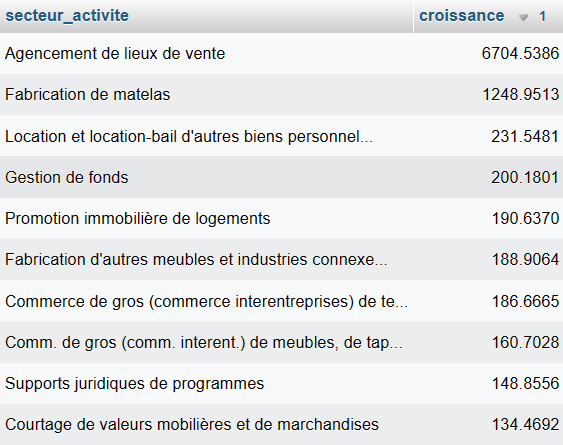
\includegraphics[width=16cm,height=9cm]{Q1.png}
\caption{Question 1.}
\end{figure}

\bigskip

\begin{itemize}
\tightlist
\item
  Description: Dans cette requête, on sélectionne la colonne secteur
  d'activite et on calcule la croissance du chiffre d'affaires entre
  2020 et 2022 en pourcentage en utilisant la formule suivante :
  ((total\_ca\_2022 - total\_ca\_2020) / total\_ca\_2020) * 100. Cela
  nous a permis de calculer le taux de croissance sur la période de 2020
  à 2022. Les résultats sont triés par ordre décroissant de croissance
  et sont limités aux 10 premiers résultats pour illustrer secteurs
  d'activité ayant connu la croissance la plus importante. \bigskip
\end{itemize}

\textbf{2)Dans quelles régions se trouvent les secteurs d'activités
ayant enregistré la plus forte croissance de chiffre d'affaires entre
2020 et 2022?} \medskip

\begin{Shaded}
\begin{Highlighting}[]
\KeywordTok{SELECT}\NormalTok{ a.secteur\_Activite, r.nom\_region, }
\NormalTok{       (e.ca\_2022 }\OperatorTok{{-}}\NormalTok{ e.ca\_2020) }\KeywordTok{AS}\NormalTok{ croissance}
\KeywordTok{FROM}\NormalTok{ Table\_Entreprise e}
\KeywordTok{JOIN}\NormalTok{ Table\_Region r }\KeywordTok{ON}\NormalTok{ e.region }\OperatorTok{=}\NormalTok{ r.nom\_region}
\KeywordTok{JOIN}\NormalTok{ table\_activite a }\KeywordTok{on}\NormalTok{ e.code\_Activite}\OperatorTok{=}\NormalTok{a.code\_Activite}
\KeywordTok{ORDER} \KeywordTok{BY}\NormalTok{ croissance }\KeywordTok{DESC}
\KeywordTok{LIMIT} \DecValTok{10}\NormalTok{;}
\end{Highlighting}
\end{Shaded}

\begin{figure}
\centering
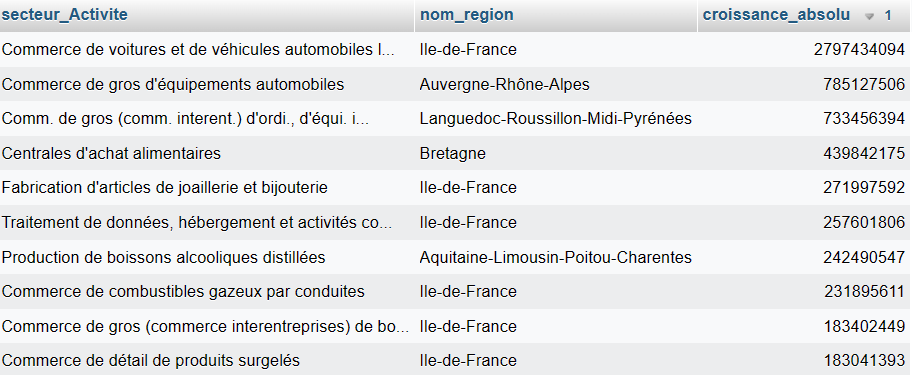
\includegraphics[width=15cm,height=10cm]{Q2.png}
\caption{Question 2.}
\end{figure}

\begin{itemize}
\tightlist
\item
  Description: Cette requête sélectionne les 10 entreprises dont la
  croissance du chiffre d'affaires entre 2020 et 2022 a été la plus
  importante. Elle relie les tables \textbf{Table\_Entreprise},
  \textbf{Table\_Region} et \textbf{Table\_Activite} pour obtenir le
  secteur d'activité de chaque entreprise ainsi que le nom de sa région.
  Le résultat de la requête affiche trois colonnes :
\end{itemize}

-``secteur\_Activite'' pour le secteur d'activité de l'entreprise
-``nom\_region'' pour le nom de la région où se situe l'entreprise
-``croissance'' pour la différence entre le chiffre d'affaires de 2022
et celui de 2020 (positif si la croissance est positive, négatif sinon)

\medskip

\textbf{3)Quels sont les secteurs d'activités qui ont enregistré les
plus gros chiffres d'affaires entre 2020 et 2022?}

\begin{Shaded}
\begin{Highlighting}[]
\KeywordTok{SELECT}\NormalTok{ secteur\_activite, }\FunctionTok{SUM}\NormalTok{(total\_ca\_2020) }\OperatorTok{+} \FunctionTok{SUM}\NormalTok{(total\_ca\_2021) }\OperatorTok{+} \FunctionTok{SUM}\NormalTok{(total\_ca\_2022) }\KeywordTok{AS}\NormalTok{ chiffre\_affaires\_total}
\KeywordTok{FROM}\NormalTok{ table\_activite}
\KeywordTok{GROUP} \KeywordTok{BY}\NormalTok{ secteur\_activite}
\KeywordTok{ORDER} \KeywordTok{BY}\NormalTok{ chiffre\_affaires\_total }\KeywordTok{DESC}
\KeywordTok{LIMIT} \DecValTok{10}\NormalTok{;}
\end{Highlighting}
\end{Shaded}

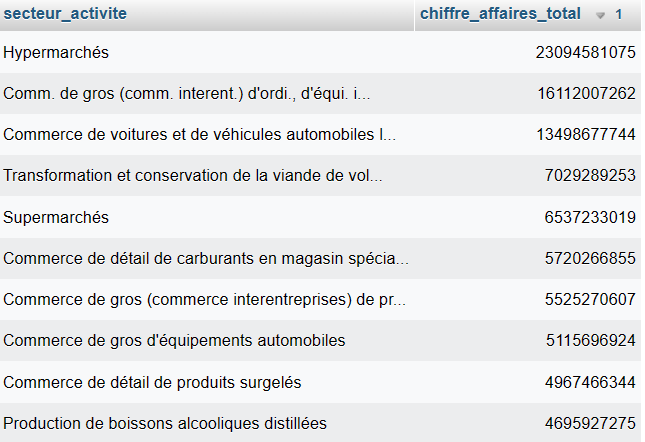
\includegraphics[width=14cm,height=11cm]{Q3.png}\bigskip

\begin{itemize}
\tightlist
\item
  Description: Cette requête SQL permet d'obtenir le chiffre d'affaires
  total pour les 10 secteurs d'activité les plus rentables en
  additionnant les chiffres d'affaires des années 2020, 2021 et 2022
  pour chaque secteur d'activité.
\end{itemize}

\bigskip

\textbf{4)Dans quelles régions se trouvent les secteurs d'activités
ayant enregistré les plus gros chiffres d'affaires au cours des trois
dernières années(2020, 2021 et 2022)? }

\begin{Shaded}
\begin{Highlighting}[]
\KeywordTok{SELECT}\NormalTok{ nom\_region, }\FunctionTok{SUM}\NormalTok{(total\_ca\_2020 }\OperatorTok{+}\NormalTok{ total\_ca\_2021 }
\OperatorTok{+}\NormalTok{ total\_ca\_2022) }\KeywordTok{AS}\NormalTok{ chiffre\_affaires\_total}
\KeywordTok{FROM}\NormalTok{ table\_region}
\KeywordTok{GROUP} \KeywordTok{BY}\NormalTok{ nom\_region}
\KeywordTok{ORDER} \KeywordTok{BY}\NormalTok{ chiffre\_affaires\_total }\KeywordTok{DESC} \KeywordTok{limit} \DecValTok{10}
\end{Highlighting}
\end{Shaded}

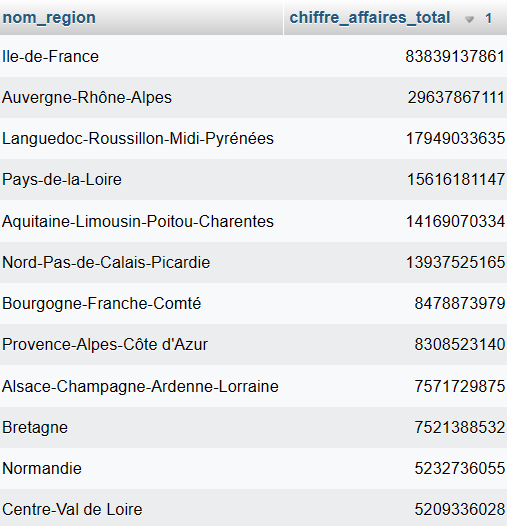
\includegraphics[width=14cm,height=11cm]{Q4.png} - Description: Cette
requête SQL permet de calculer le chiffre d'affaires total par région en
additionnant les chiffres d'affaires des années 2020, 2021 et 2022 de
toutes les entreprises de chaque région, puis en triant les résultats
par ordre décroissant de chiffre d'affaires total.

\large
\enspace

\textbf{5)Quelles sont les régions où se trouvent les entreprises ayant
le plus gros chiffre d'affaires sur les trois dernières années(2020,
2021, 2022)? }

\begin{Shaded}
\begin{Highlighting}[]
\KeywordTok{SELECT}\NormalTok{ region, }
       \FunctionTok{MAX}\NormalTok{(total\_ca\_2022) }\KeywordTok{AS}\NormalTok{ ca\_2022, }
       \FunctionTok{MAX}\NormalTok{(total\_ca\_2021) }\KeywordTok{AS}\NormalTok{ ca\_2021, }
       \FunctionTok{MAX}\NormalTok{(total\_ca\_2020) }\KeywordTok{AS}\NormalTok{ ca\_2020 }
\KeywordTok{FROM}\NormalTok{ Table\_Region,table\_entreprise }
\KeywordTok{where}\NormalTok{ Table\_Region.nom\_region }\OperatorTok{=}\NormalTok{ Table\_Entreprise.region }
\KeywordTok{GROUP} \KeywordTok{BY}\NormalTok{ region }
\KeywordTok{ORDER} \KeywordTok{BY}\NormalTok{ ca\_2022 }\KeywordTok{DESC}\NormalTok{, ca\_2021 }\KeywordTok{DESC}\NormalTok{, ca\_2020 }\KeywordTok{DESC} 
\KeywordTok{LIMIT} \DecValTok{10}\NormalTok{;}
\end{Highlighting}
\end{Shaded}

\begin{figure}
\centering
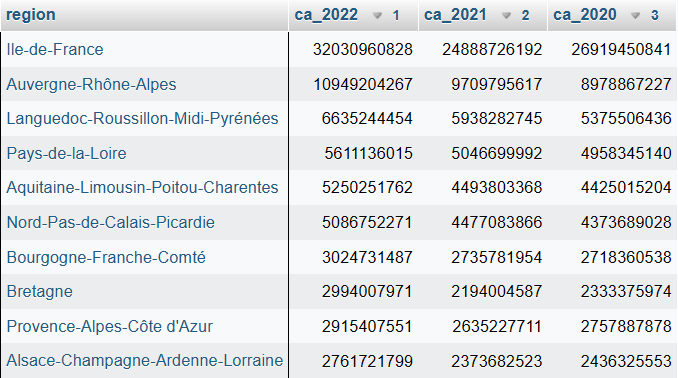
\includegraphics[width=15cm,height=10cm]{Q5.png}
\caption{Question 5.}
\end{figure}

\medskip

Cette requête récupère les 10 régions ayant le plus grand chiffre
d'affaires en 2022, 2021 et 2020, en prenant les données des tables
Table\_Region et Table\_Entreprise. La clause \textbf{where} permet de
faire la jointure entre les deux tables sur le champ nom\_region de
Table\_Region et region de Table\_Entreprise. Les colonnes renvoyées
sont region pour le nom de la région, ca\_2022 pour le chiffre
d'affaires total de l'année 2022, ca\_2021 pour le chiffre d'affaires
total de l'année 2021, et ca\_2020 pour le chiffre d'affaires total de
l'année 2020. Le chiffre d'affaires total est obtenu en calculant la
somme des chiffres d'affaires des entreprises de chaque région.

\medskip

Dans cette requête, on utilise une jointure entre les tables
Table\_Region et Table\_Entreprise pour regrouper les entreprises par
région,puis on a calculé le chiffre d'affaire total pour chaque année.
Ensuite, on a effectué la sélection des régions avec le chiffre
d'affaires le plus élevé pour chaque année en utilisant la fonction
d'agrégation \textbf{MAX}.Enfin,on ordonne les résultats par chiffre
d'affaires décroissant en affichant que les résultats des 10 premières
régions.

\bigskip

\hypertarget{matuxe9riel-et-muxe9thodes}{%
\chapter{Matériel et Méthodes}\label{matuxe9riel-et-muxe9thodes}}

\hypertarget{logiciels}{%
\section{Logiciels}\label{logiciels}}

Notre outil principal pour se communiquer entre les membres du groupe
est le discord(utilisation de snapchat au debut) ou BBB sur mooodle. On
a partagé toutes nos données et toutes les informations importante
concernant le projet. Ensuite, On a utilisé Excel pour l'uniformisation
des données et le filtrage des colonnes. La bibliothèque Pandas de
python a été d'une grande aide pour le néttoyage complet des données
bien vraie que le logiciel nous a aussi bien aidé au debut sur le
nettoyage de données. En plus R,a été utilisé pour mettre en relation
tous les logiciels notamment notre base de données, puis produire ce
rapport final(via RMarkdown). Enfin, on a utilisé phpMyAdmin pour
réalisé des requêtes sur notre base de données. \enspace Voici les
informations sur les versions des logiciels et sur l'ordinateur qui a
servi pour les analyses. \medskip

\begin{itemize}
\tightlist
\item
  Ordinateur:

  \begin{itemize}
  \tightlist
  \item
    Nom de l'appareil: \textbf{LAPTOP-KTKJ2BP4}
  \item
    Processeur: \textbf{Intel(R) Core(TM) i7-1065G7 CPU @ 1.30GHz 1.50
    GHz}
  \item
    Memoire Ram installé: \textbf{8,00Go (7,74Go utilisable)}
  \item
    Type du sytéme: \textbf{Système d'exploitation 64bits, processeur
    x64}
  \item
    Marque: ASUS
  \end{itemize}
\item
  Python:

  \begin{itemize}
  \tightlist
  \item
    version: 3.9.12
  \item
    google Collab -jupyter(avec anaconda)
  \end{itemize}
\item
  R:

  \begin{itemize}
  \tightlist
  \item
    platform: x86\_64-w64-mingw32\\
  \item
    arch: x86\_64\\
  \item
    os: mingw32\\
  \item
    crt: ucrt\\
  \item
    system: x86\_64, mingw32\\
  \item
    status\\
  \item
    major: 4\\
  \item
    minor: 3.0\\
  \item
    year: 2023\\
  \item
    month: 04\\
  \item
    day: 21\\
  \item
    svn rev: 84292\\
  \item
    language: R\\
  \item
    version.string R version: 4.3.0 (2023-04-21 ucrt)
  \item
    nickname: Already Tomorrow
  \end{itemize}
\end{itemize}

Listons tous les logiciels utiliser pour la partie Base de Données,
statistique mais également pour gérer et communiquer entre les membres
du projet. \medskip On a privilégié les logiciels R (ou Python) pour la
Science des Données. Pour assurer une reproductibilité maximale, on a
utiliser R Markdown,via RStudio. \bigskip \#\# Description des Données
\# lister toutes les connexions actives

\textbf{- Comment les données sont-elles stockées?} Les données ont été
tiré dans un fichier CSV(nommé chiffre clé),puis on les a néttoyé et
stocké dans une base de données sql dans phpMyAdmin. Ce qui nous a
permis d'effectuer des requêtes SQL et par la suite recupérer les
données pour pouvoir faire des analyses statistiques.

\textbf{- Quelles sont les tailles des fichiers en jeu? Combien y a t-il
de fichiers?}

Notre fichier avant l'utilisation etait de 67 643 ko contenant 167 885
lignes et 42 colonnes.On a utiliser un seul fichier(chiffre clé 2022)
pour l'extraction des données car on a juger que les autres n'étaient
pas necessaire, vu notre problématqiue posées.

\textbf{- Combien d'unités statistiques? Combien de variables? etc.}
Notre base de données contient trois tables.Voici les informations pour
chacune des tables : \medskip -Table\_Activite: 443 unités statistiques
et 5 variables \medskip -Table\_Entreprise: 3,264 unités statistiques et
11 variables \medskip -Table\_Region: 17 unités statistiques et 4
variables \medskip En total, notre base de données contient \textbf{3
724 unités statistiques} et \textbf{20 variables}.

\hypertarget{nettoyage-des-donnuxe9es}{%
\section{Nettoyage des données}\label{nettoyage-des-donnuxe9es}}

Comment gérez-vous les données manquantes, etc. ?

Pour gérer les données manquantes, on a utilisé des fonctions SQL pour
filtrer les enregistrements qui contiennent des valeurs manquantes ou
pour remplacer les valeurs manquantes par des valeurs par défaut. On a
également utilisé des fonctions de traitement de chaînes de caractères
avec le logiciel R(données paramétrées avec l'encodage utf-8 pour les
rendre plus visible) ou python(Pandas, Numpy,..) pour nettoyer les
données en supprimant les espaces inutiles, les caractères spéciaux,
etc.

\hypertarget{uxe9tapes-de-pruxe9-traitements}{%
\section{Étapes de
Pré-traitements}\label{uxe9tapes-de-pruxe9-traitements}}

\textbf{-Quelles transformations avez-vous effectuées sur vos données
pour les rendre utilisables?}

\begin{itemize}
\tightlist
\item
  Pour rendre les données utilisables, on a effectué des transformations
  telles que la normalisation des données, la discrétisation des
  variables continues, la transformation des variables catégorielles en
  variables binaires, etc. Ces transformations ont été effectué à l'aide
  de fonctions SQL ou de bibliothèques de traitement de données en R ou
  Python.
\item
  On a également explorer les données à l'aide de graphiques et de
  résumés statistiques pour identifier des schémas et des tendances, et
  pour valider la qualité des données avant d'effectuer des analyses
\end{itemize}

\hypertarget{moduxe9lisation-statistique}{%
\section{Modélisation statistique}\label{moduxe9lisation-statistique}}

Quels outils ou méthodes de statistiques allez-vous utiliser? Donner des
équations mathématiques sMil y a lieu et lister les éventuels
présupposés («assumptions» en anglais) que vous devez faire sur les
données afin d'utiliser ces outils ou méthodes (\emph{e.g.}, normalité,
absence de valeurs aberrantes, etc.).

Il est également bon d'indiquer quelles sont les avantages et les
limites de ces méthodes.

Vous pourrez consulter avec profit les Chapitre 11--13 du livre sur R
utilisé pendant le cours :

\url{http://biostatisticien.eu/springeR/livreR.pdf}

\hypertarget{analyse-exploratoire-des-donnuxe9es}{%
\chapter{Analyse Exploratoire des
Données}\label{analyse-exploratoire-des-donnuxe9es}}

Toute étude impliquant des données doit \textbf{obligatoirement} inclure
une analyse exploratoire préalable. Celle-ci permet de mieux comprendre
l'information contenue dans les données. De ce fait,cette partie a pour
but de mieux comprendre l'information contenue dans nos données, pour
cela nous avons généré différents graphiques et plusieurs valeurs
numériques. Ainsi, pour faire des analyses pertinentes nous avons
décider de se poser certains bon nombre de questions, afin de répondre à
notre problématique. Ces questions vont répondre sur l'analyse de la
performance économique des différentes régions et secteurs d'activités
au cours des trois dernières années(2020, 2021, 2022). Elles permettront
d'identifier les tendances et les modèles dans les données, de comparer
les performances des différentes régions et secteurs, et de prendre des
décisions éclairées en matière d'investissement et de gestion
financière. Voici nos questions:

-Quels sont les secteurs d'activités ayant enregistré la plus forte
croissance de chiffre d'affaires au cours des trois dernières
années(2020, 2021, 2022)?

-Dans quelles région se trouvent les secteurs d'activités ayant
enregistré la plus forte croissance de chiffre d'affaires au cours des
trois dernières années(2020, 2021, 2022)?

-Quels sont les secteurs d'activités qui ont enregistré les plus gros
chiffres d'affaires au cours des trois dernières années(2020, 2021,
2022)?

-Dans quelles régions se trouvent les secteurs d'activités ayant
enregistré les plus gros chiffres d'affaires au cours des trois
dernières années(2020, 2021, 2022)?

\hypertarget{resumuxe9-des-donnuxe9es}{%
\section{\texorpdfstring{\textbf{Resumé des
données}}{Resumé des données}}\label{resumuxe9-des-donnuxe9es}}

On utilise la fonction summary pour obtenir un résumé statistique des
données sur nos entreprises. Cela nous permettra d'avoir rapidement un
aperçu sur les données tel que les chiffres d'affaires des entreprises
en 2022 qui nous intéresse ici. \medskip \textbf{Resumé des données de
la table entreprise:} \medskip

\bigskip

\begin{Shaded}
\begin{Highlighting}[]
\KeywordTok{SELECT} \OperatorTok{*} 
\KeywordTok{from}\NormalTok{ table\_entreprise}
\end{Highlighting}
\end{Shaded}

\begin{figure}
\centering
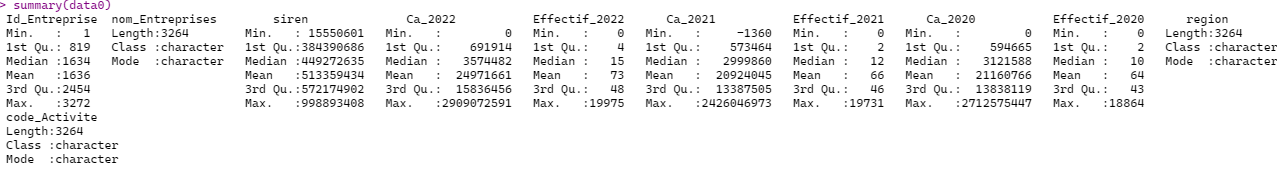
\includegraphics[width=10cm,height=5cm]{Resume.png}
\caption{Diagramme en barre vertical.}
\end{figure}

\begin{Shaded}
\begin{Highlighting}[]
\FunctionTok{summary}\NormalTok{(var2)}
\end{Highlighting}
\end{Shaded}

\textbf{Résumé des chiffres d'affaire des entreprises en 2022:}

\begin{Shaded}
\begin{Highlighting}[]
\FunctionTok{summary}\NormalTok{(var2}\SpecialCharTok{$}\NormalTok{Ca\_2022)}
\end{Highlighting}
\end{Shaded}

\begin{verbatim}
##      Min.   1st Qu.    Median      Mean   3rd Qu.      Max. 
## 0.000e+00 6.919e+05 3.574e+06 2.497e+07 1.584e+07 2.909e+09
\end{verbatim}

\medskip

Voici un résumé des informations obtenues à partir de l'analyse des
chiffres d'affaires des entreprises en 2022 :

\begin{itemize}
\item
  La \textbf{moyenne} de chiffre d'affaires en 2022 est de \textbf{24
  971 661 euros}. Cela signifie que si l'on additionne tous les chiffres
  d'affaires de toutes les entreprises et que l'on divise cette somme
  par le nombre total d'entreprises, on obtient une moyenne de 24 971
  661. Cependant, il est important de noter que la moyenne peut être
  biaisée par des valeurs extrêmes (appelées ``outliers''), ce qui peut
  fausser la représentativité de cette mesure. C'est pourquoi il ce
  serait mieux d'utiliser d'autres mesures de tendance centrale en
  combinaison avec la moyenne, comme la médiane ou le mode.
\item
  Le chiffre d'affaires \textbf{minimum} est \textbf{de 0 euro}, ce qui
  pourrait être dû à des entreprises qui n'ont pas généré de revenus au
  cours de cette période.
\item
  Le \textbf{premier quartile} est de \textbf{691 914 euros}, ce qui
  signifie que \textbf{25\%} des entreprises ont un chiffre d'affaires
  inférieur à ce montant.
\item
  La \textbf{médiane}, qui est la valeur au milieu de la distribution,
  est de \textbf{3 574 482 euros}. Cela signifie que 50\% des
  entreprises ont un chiffre d'affaires inférieur à ce montant et 50\%
  ont un chiffre d'affaires supérieur.
\item
  Le \textbf{troisième quartile} est de \textbf{15 836 456 euros}, ce
  qui signifie que 75\% des entreprises ont un chiffre d'affaires
  inférieur à ce montant.
\item
  La valeur \textbf{maximale} de chiffre d'affaires est de \textbf{2 909
  072 591 euros}, ce qui représente l'entreprise ayant généré le plus de
  revenus en \textbf{2022}.
\end{itemize}

\textbf{Ecart-type(sd) et Variance(var)}

\begin{Shaded}
\begin{Highlighting}[]
\CommentTok{\#Variance}
\FunctionTok{var}\NormalTok{(var2}\SpecialCharTok{$}\NormalTok{Ca\_2022)}
\end{Highlighting}
\end{Shaded}

\begin{verbatim}
## [1] 1.405396e+16
\end{verbatim}

\begin{Shaded}
\begin{Highlighting}[]
\CommentTok{\#ecartype}
\FunctionTok{sd}\NormalTok{(var2}\SpecialCharTok{$}\NormalTok{Ca\_2022)}
\end{Highlighting}
\end{Shaded}

\begin{verbatim}
## [1] 118549414
\end{verbatim}

\medskip

La variance (var) est une mesure de dispersion qui calcule la moyenne
des carrés des écarts à la moyenne d'un échantillon de données. Elle est
définie comme la différence entre la moyenne des carrés et le carré de
la moyenne de l'échantillon. Plus la variance est grande, plus les
données sont dispersées autour de la moyenne.Dans nos données la valeur
du chiffre d'affaire 2022 est très élevée (environ 1.4e+16), ce qui
indique que les données ont une grande dispersion autour de la moyenne.
La déviation standard (sd) ou ecart-type, quant à elle, est une mesure
de la dispersion qui calcule la racine carrée de la variance. Elle est
utilisée pour mesurer la variation des données par rapport à leur
moyenne. La valeur du chiffre d'affaire en 2022 est d'environ 118 549
414, ce qui indique que les données ont une variation relativement
élevée par rapport à leur moyenne.

\bigskip

\hypertarget{ruxe9ponses-aux-questions-uxe0-laide-de-r}{%
\section{\texorpdfstring{\textbf{Réponses aux Questions à l'aide de
R}}{Réponses aux Questions à l'aide de R}}\label{ruxe9ponses-aux-questions-uxe0-laide-de-r}}

\medskip

\textbf{1)Quels sont les secteurs d'activités qui ont enregistré la plus
forte croissance entre 2020 et 2022 ?}

\medskip

\begin{figure}
\centering
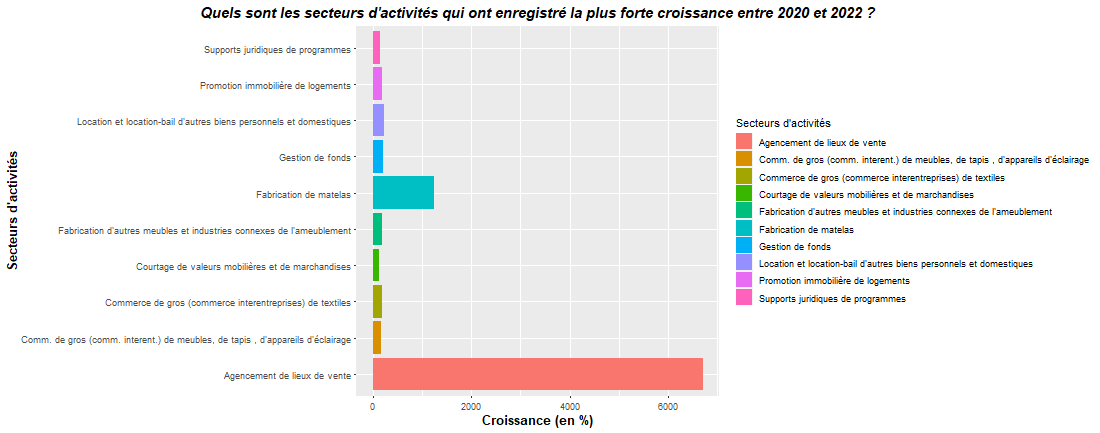
\includegraphics[width=15cm,height=8cm]{graphique_requete1.png}
\caption{Diagramme en barre.}
\end{figure}

\medskip

Le graphique affiche les 10 secteurs d'activités avec la plus forte
croissance de revenus entre 2020 et 2022 en France. Comme nous pouvons
le voir sur le graphique, parmi les 10 secteurs d'activités avec le taux
de croissance le plus élevé, 2 secteurs prédominent. Le secteur de
\textbf{fabrication de matelas} a enregistré une croissance d'environ
\textbf{1249\%} entre 2020 et 2022 mais c'est surtout le secteur
\textbf{d'agencement de lieux de vente} qui a connu une forte
augmentation du taux de croissance d'environ \textbf{6705\%} sur la même
période. Cela est probablement du à la crise du Covid-19 qui a eu lieu
en 2020.

\bigskip

\textbf{2)Dans quelles régions se trouvent les secteurs d'activités
ayant enregistré la plus forte croissance de chiffre d'affaires entre
2020 et 2022?}

\medskip

\begin{figure}
\centering
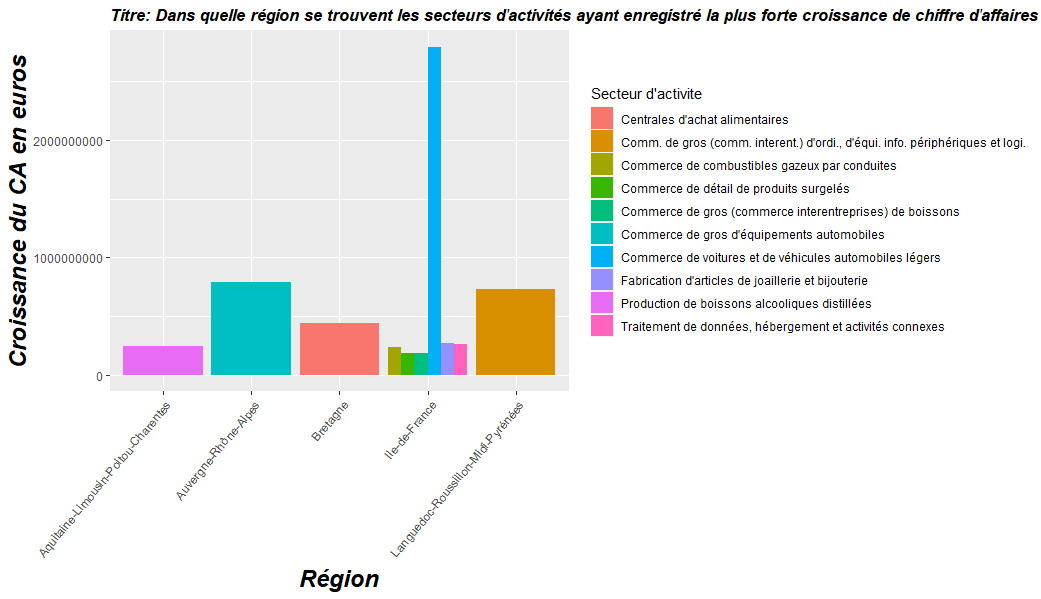
\includegraphics[width=15cm,height=8cm]{graphique_requete2.png}
\caption{Diagramme en barre des régions où on trouvent les secteurs
d'activités avec la plus forte croissance entre 2020 et 2022.}
\end{figure}

\medskip

Ce graphe permet de répondre à la question ``Dans quelle région se
trouvent les secteurs d'activités ayant enregistré la plus forte
croissance de chiffre d'affaires au cours des trois dernières
années(2020 à 2022)?''. Il affiche la répartition par région sous forme
de diagramme en barre avec la croissance du CA en tant que poids. Cela
permet de visualiser les régions où les secteurs d'activités connaissant
la croissance la plus rapide en termes de CA et de comprendre les
tendances et les opportunités de croissance potentielles pour les
entreprises dans ces régions et secteurs.

\bigskip

\textbf{3)Quels sont les secteurs d'activités qui ont enregistré les
plus gros chiffres d'affaires au cours des trois dernières années?}
\bigskip

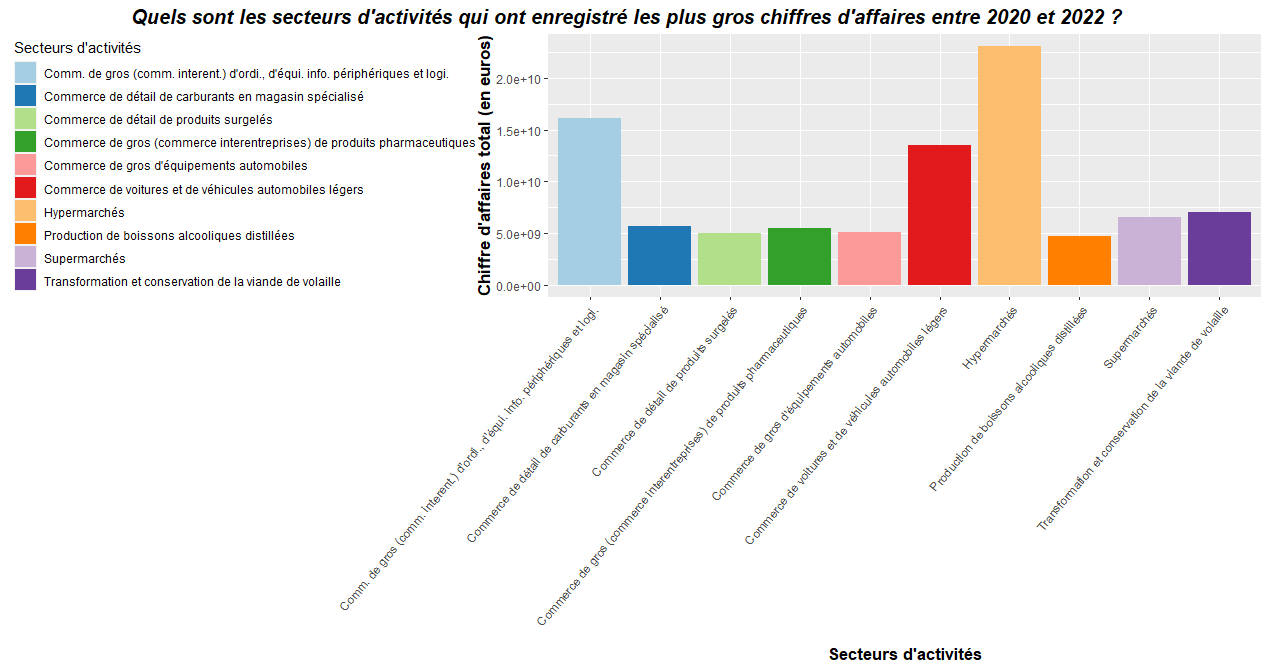
\includegraphics[width=15cm,height=8cm]{graphique_requete3.png} Le
graphique affiche les 10 secteurs d'activités avec les plus gros
chiffres d'affaires entre 2020 et 2022 en France. Nous remarquons sur le
graphique, 3 secteurs d'activités qui ont accumulé plus de 10 milliards
d'euros de chiffres d'affaires entre 2020 et 2022. Le \textbf{commerce
de voitures et de véhicules automobile} a engendré plus de \textbf{13
milliards d'euros} durant cette période. Quant au commerce de gros
d'ordinateurs, d'équipements informatiques, il a amené plus de
\textbf{16 milliards d'euros} de chiffre d'affaires. Les
\textbf{hypermarchés} sont les premiers secteurs d'activités, ils ont
rapporté plus de \textbf{23 milliards d'euros} de chiffre d'affaires en
France ces 3 dernières années.

\textbf{4)Dans quelles régions se trouvent les secteurs d'activités
ayant enregistré les plus gros chiffres d'affaires au cours des trois
dernières années? }

\begin{figure}
\centering
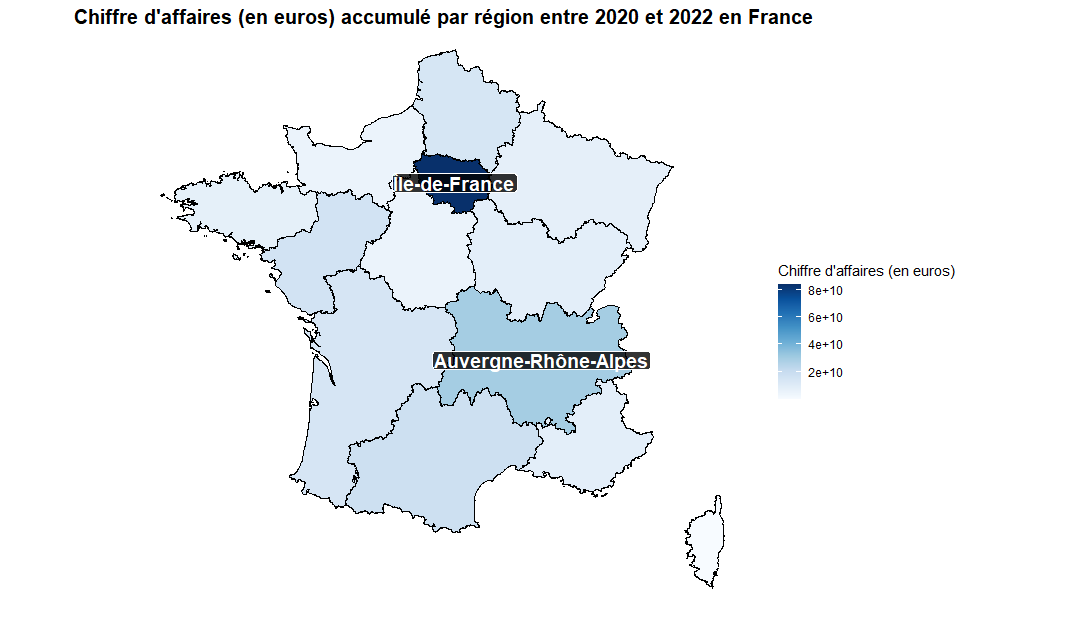
\includegraphics[width=15cm,height=8cm]{graphique_requete4.png}
\caption{Carte.}
\end{figure}

Le graphique montre les différentes régions de France selon le chiffre
d'affaires qu'elles ont obtenu. La deuxième région qui a accumulé le
plus de chiffres d'affaires est la région \textbf{Auvergne-Rhône-Alpes}
qui a généré plus de \textbf{29 milliars d'euros} entre 2020 et 2022.
C'est beaucoup moins que la région \textbf{Île-de-France (bleu foncé sur
le graphique)} qui a engendré environ \textbf{84 milliars d'euros} de
chiffres d'affaires soit presque 3 fois plus que la région
\textbf{Auvergne-Rhône-Alpes}. \textbf{NB}: Nous avons laissé seulement
la France métropolitaine pour avoir un graphique plus clair. \bigskip

\hypertarget{conclusion-et-perspectives}{%
\chapter{Conclusion et perspectives}\label{conclusion-et-perspectives}}

Pour conclure, nous pensons pouvoir proposer deux types d'investissement
sur les secteurs d'activités.

La première, serait d'investir dans les secteurs ayant eu une forte
évolution de leurs chiffres d'affaires sur les trois dernières années.
Nos analyses nous permettent d'avoir les deux secteurs remplissant le
plus cette condition: « Courtage de valeurs mobilières et de
marchandises'' et ``Transformation et conservation de poisson ».

La deuxième stratégie d'investissement serait d'investir dans les
domaines d'activités qui génèrent le plus de chiffre d'affaires. Ces
secteurs sont les plus stables sur le long terme car leurs chiffres
d'affaires restent élevés même s'ils ne présentent pas de grosses
évolutions sur les 3 années étudiées. Les trois secteurs qui ressortent
le plus sont « hypermarchés », « transformation et conservation de
volaille » et « commerce de voitures et de véhicules automobiles légers
».

Dans une prochaine étude, il serait intéressant d'analyser les secteurs
avec la plus grosse croissance sur ces trois dernières années pour voir
si les résultats restent cohérents avec ceux obtenus cette année pour en
conclure le retour positif de notre investissement

\hypertarget{bibliographie}{%
\chapter*{Bibliographie}\label{bibliographie}}
\addcontentsline{toc}{chapter}{Bibliographie}

\leavevmode\vadjust pre{\hypertarget{refs}{}}%
\begin{CSLReferences}{0}{0}
\url{https://www.data-to-viz.com/}
\url{https://www.data.gouv.fr/fr/datasets/base-sirene-des-entreprises-et-de-leurs-etablissements-siren-siret/}
\url{https://www.data.gouv.fr/fr/datasets/chiffres-cles-2022/}

\end{CSLReferences}

\bibliographystyle{elsarticle-harv}
\bibliography{references}

\hypertarget{annexes}{%
\chapter*{Annexes}\label{annexes}}
\addcontentsline{toc}{chapter}{Annexes}

Il faut utiliser les annexes de façon judicieuse. C'est ici que l'on
place des résultats trop volumineux pour apparaître dans le corps du
rapport. Ou bien des résultats (e.g., graphiques) moins intéressants que
les autres. Cela permet de limiter le nombre de pages du coeur du
rapport, et d'ajouter des détails dans cette partie pour le lecteur
désireux d'en savoir plus.

\hypertarget{codes}{%
\section*{\texorpdfstring{\textbf{Codes}}{Codes}}\label{codes}}
\addcontentsline{toc}{section}{\textbf{Codes}}

Ajouter vos codes informatiques ici. Les codes doivent être correctement
indentés et commentés. \textbf{connexion à notre base de données}

\begin{Shaded}
\begin{Highlighting}[]
\FunctionTok{library}\NormalTok{(DBI)}
\FunctionTok{library}\NormalTok{(RMySQL)}
\NormalTok{conn }\OtherTok{\textless{}{-}}\NormalTok{ DBI}\SpecialCharTok{::}\FunctionTok{dbConnect}\NormalTok{(RMySQL}\SpecialCharTok{::}\FunctionTok{MySQL}\NormalTok{(), }
                  \AttributeTok{user =} \StringTok{"BDD\_arrivedirt"}\NormalTok{, }
                  \AttributeTok{password =} \StringTok{"df50a60dc58cfb65eefe321dcd88a5168dfd5083"}\NormalTok{, }
                  \AttributeTok{dbname =} \StringTok{"BDD\_arrivedirt"}\NormalTok{, }
                  \AttributeTok{host =} \StringTok{"60d.h.filess.io"}\NormalTok{,}
                \AttributeTok{port=}\DecValTok{3307}\NormalTok{)}
\FunctionTok{dbListTables}\NormalTok{(conn)}
\end{Highlighting}
\end{Shaded}

\begin{itemize}
\tightlist
\item
  \textbf{Partie base de données}
\end{itemize}

\textbf{1)Quels sont les secteurs d'activités ayant enregistré la plus
forte croissance de chiffre d'affaires au cours des trois dernières
années(2020,2021,2022)?}

\bigskip

\begin{Shaded}
\begin{Highlighting}[]
\KeywordTok{SELECT}\NormalTok{ secteur\_activite,}
\NormalTok{((total\_ca\_2022 }\OperatorTok{{-}}\NormalTok{ total\_ca\_2020)}\OperatorTok{/}\NormalTok{total\_ca\_2020)}\OperatorTok{*}\DecValTok{100} \KeywordTok{AS}\NormalTok{ croissance}
\KeywordTok{FROM}\NormalTok{ table\_activite}
\KeywordTok{ORDER} \KeywordTok{BY}\NormalTok{ croissance }\KeywordTok{DESC}
\KeywordTok{LIMIT} \DecValTok{10}\NormalTok{;}\OtherTok{"}
\end{Highlighting}
\end{Shaded}

\textbf{2)Dans quelles régions se trouvent les secteurs d'activités
ayant enregistré la plus forte croissance de chiffre d'affaires entre
2020 et 2022?} \medskip

\begin{Shaded}
\begin{Highlighting}[]
\KeywordTok{SELECT}\NormalTok{ a.secteur\_Activite, r.nom\_region, }
\NormalTok{       (e.ca\_2022 }\OperatorTok{{-}}\NormalTok{ e.ca\_2020) }\KeywordTok{AS}\NormalTok{ croissance}
\KeywordTok{FROM}\NormalTok{ Table\_Entreprise e}
\KeywordTok{JOIN}\NormalTok{ Table\_Region r }\KeywordTok{ON}\NormalTok{ e.region }\OperatorTok{=}\NormalTok{ r.nom\_region}
\KeywordTok{JOIN}\NormalTok{ table\_activite a }\KeywordTok{on}\NormalTok{ e.code\_Activite}\OperatorTok{=}\NormalTok{a.code\_Activite}
\KeywordTok{ORDER} \KeywordTok{BY}\NormalTok{ croissance }\KeywordTok{DESC}
\KeywordTok{LIMIT} \DecValTok{10}\NormalTok{;}
\end{Highlighting}
\end{Shaded}

\medskip

\textbf{3)Quels sont les secteurs d'activités qui ont enregistré les
plus gros chiffres d'affaires entre 2020 et 2022?}

\begin{Shaded}
\begin{Highlighting}[]
\KeywordTok{SELECT}\NormalTok{ secteur\_activite, }\FunctionTok{SUM}\NormalTok{(total\_ca\_2020) }\OperatorTok{+} \FunctionTok{SUM}\NormalTok{(total\_ca\_2021) }\OperatorTok{+} \FunctionTok{SUM}\NormalTok{(total\_ca\_2022) }\KeywordTok{AS}\NormalTok{ chiffre\_affaires\_total}
\KeywordTok{FROM}\NormalTok{ table\_activite}
\KeywordTok{GROUP} \KeywordTok{BY}\NormalTok{ secteur\_activite}
\KeywordTok{ORDER} \KeywordTok{BY}\NormalTok{ chiffre\_affaires\_total }\KeywordTok{DESC}
\KeywordTok{LIMIT} \DecValTok{10}\NormalTok{;}
\end{Highlighting}
\end{Shaded}

\bigskip

\textbf{4)Dans quelles régions se trouvent les secteurs d'activités
ayant enregistré les plus gros chiffres d'affaires au cours des trois
dernières années(2020, 2021 et 2022)? }

\begin{Shaded}
\begin{Highlighting}[]
\KeywordTok{SELECT}\NormalTok{ nom\_region, }\FunctionTok{SUM}\NormalTok{(total\_ca\_2020 }\OperatorTok{+}\NormalTok{ total\_ca\_2021 }
\OperatorTok{+}\NormalTok{ total\_ca\_2022) }\KeywordTok{AS}\NormalTok{ chiffre\_affaires\_total}
\KeywordTok{FROM}\NormalTok{ table\_region}
\KeywordTok{GROUP} \KeywordTok{BY}\NormalTok{ nom\_region}
\KeywordTok{ORDER} \KeywordTok{BY}\NormalTok{ chiffre\_affaires\_total }\KeywordTok{DESC} \KeywordTok{limit} \DecValTok{10}
\end{Highlighting}
\end{Shaded}

\bigskip

\begin{itemize}
\tightlist
\item
  \textbf{Partie Science de données}\bigskip
\end{itemize}

\textbf{1)Quels sont les secteurs d'activités qui ont enregistré la plus
forte croissance entre 2020 et 2022 ?}

\begin{Shaded}
\begin{Highlighting}[]
\NormalTok{requete1 }\OtherTok{\textless{}{-}} \StringTok{"SELECT secteur\_activite,}
\StringTok{((total\_ca\_2022 {-} total\_ca\_2020)/total\_ca\_2020)*100 AS croissance}
\StringTok{FROM table\_activite}
\StringTok{ORDER BY croissance DESC}
\StringTok{LIMIT 10;"}
\NormalTok{requete1}
\FunctionTok{View}\NormalTok{(requete1)}
\NormalTok{data1 }\OtherTok{\textless{}{-}} \FunctionTok{dbGetQuery}\NormalTok{(bd, requete1)}

\FunctionTok{ggplot}\NormalTok{(data1) }\SpecialCharTok{+}
  \FunctionTok{aes}\NormalTok{(}
    \AttributeTok{x =}\NormalTok{ secteur\_activite,}
    \AttributeTok{fill =}\NormalTok{ secteur\_activite,}
    \AttributeTok{weight =}\NormalTok{ croissance}
\NormalTok{  ) }\SpecialCharTok{+}
  \FunctionTok{geom\_bar}\NormalTok{(}\AttributeTok{position =} \StringTok{"dodge"}\NormalTok{) }\SpecialCharTok{+}
  \FunctionTok{scale\_fill\_hue}\NormalTok{(}\AttributeTok{direction =} \DecValTok{1}\NormalTok{) }\SpecialCharTok{+}
  \FunctionTok{labs}\NormalTok{(}
    \AttributeTok{x =} \StringTok{"Secteurs d\textquotesingle{}activités"}\NormalTok{,}
    \AttributeTok{y =} \StringTok{"Croissance (en \%)"}\NormalTok{,}
    \AttributeTok{title =} \StringTok{"Quels sont les secteurs d\textquotesingle{}activités qui ont enregistré la plus forte croissance entre 2020 et 2022 ?"}\NormalTok{,}
    \AttributeTok{fill =} \StringTok{"Secteurs d\textquotesingle{}activités"}
\NormalTok{  ) }\SpecialCharTok{+}
  \FunctionTok{coord\_flip}\NormalTok{() }\SpecialCharTok{+}
  \FunctionTok{theme\_gray}\NormalTok{() }\SpecialCharTok{+}
  \FunctionTok{theme}\NormalTok{(}
    \AttributeTok{plot.title =} \FunctionTok{element\_text}\NormalTok{(}\AttributeTok{size =}\NormalTok{ 15L,}
                              \AttributeTok{face =} \StringTok{"bold.italic"}\NormalTok{,}
                              \AttributeTok{hjust =} \FloatTok{0.5}\NormalTok{),}
    \AttributeTok{axis.title.y =} \FunctionTok{element\_text}\NormalTok{(}\AttributeTok{size =}\NormalTok{ 13L,}
                                \AttributeTok{face =} \StringTok{"bold"}\NormalTok{),}
    \AttributeTok{axis.title.x =} \FunctionTok{element\_text}\NormalTok{(}\AttributeTok{size =}\NormalTok{ 13L,}
                                \AttributeTok{face =} \StringTok{"bold"}\NormalTok{)}
\NormalTok{  )}
\end{Highlighting}
\end{Shaded}

\medskip

\textbf{2)Dans quelles régions se trouvent les secteurs d'activités
ayant enregistré la plus forte croissance de chiffre d'affaires entre
2020 et 2022?}

\begin{Shaded}
\begin{Highlighting}[]
\NormalTok{   diagramme }\OtherTok{=} \FunctionTok{ggplot}\NormalTok{(data3) }\SpecialCharTok{+}
  \FunctionTok{aes}\NormalTok{(}
    \AttributeTok{x =}\NormalTok{ nom\_region,}
    \AttributeTok{fill =}\NormalTok{ secteur\_Activite,}
    \AttributeTok{weight =}\NormalTok{ croissance}
\NormalTok{  ) }\SpecialCharTok{+}
  \FunctionTok{geom\_bar}\NormalTok{(}\AttributeTok{position =} \StringTok{"dodge"}\NormalTok{) }\SpecialCharTok{+}
  \FunctionTok{scale\_fill\_hue}\NormalTok{(}\AttributeTok{direction =} \DecValTok{1}\NormalTok{) }\SpecialCharTok{+}
  \FunctionTok{labs}\NormalTok{(}
    \AttributeTok{x =} \StringTok{"Région"}\NormalTok{,}
    \AttributeTok{y =} \StringTok{"Croissance du CA en millons d\textquotesingle{}euros"}\NormalTok{,}
    \AttributeTok{title =} \StringTok{"Titre: Dans quelle région se trouvent les secteurs d\textquotesingle{}activités }
\StringTok{    ayant enregistré la plus forte croissance de chiffre d\textquotesingle{}affaires entre }
\StringTok{    2020 et 2022?"}\NormalTok{,}
    \AttributeTok{fill =} \StringTok{"Secteur d\textquotesingle{}activite"}
\NormalTok{  ) }\SpecialCharTok{+}
  \FunctionTok{theme\_gray}\NormalTok{() }\SpecialCharTok{+}
  \FunctionTok{theme}\NormalTok{(}
    \AttributeTok{plot.title =} \FunctionTok{element\_text}\NormalTok{(}\AttributeTok{face =} \StringTok{"bold.italic"}\NormalTok{),}
    \AttributeTok{plot.subtitle =} \FunctionTok{element\_text}\NormalTok{(}\AttributeTok{size =}\NormalTok{ 14L,}
    \AttributeTok{face =} \StringTok{"italic"}\NormalTok{,}
    \AttributeTok{hjust =} \FloatTok{0.5}\NormalTok{),}
    \AttributeTok{axis.title.y =} \FunctionTok{element\_text}\NormalTok{(}\AttributeTok{size =}\NormalTok{ 18L,}
    \AttributeTok{face =} \StringTok{"bold.italic"}\NormalTok{),}
    \AttributeTok{axis.title.x =} \FunctionTok{element\_text}\NormalTok{(}\AttributeTok{size =}\NormalTok{ 18L,}
    \AttributeTok{face =} \StringTok{"bold.italic"}\NormalTok{)}
\NormalTok{  ) }
\end{Highlighting}
\end{Shaded}

\medskip

\textbf{3)Quels sont les secteurs d'activités qui ont enregistré les
plus gros chiffres d'affaires au cours des trois dernières années?}

\begin{Shaded}
\begin{Highlighting}[]
\NormalTok{requete2 \textless{}{-} SELECT secteur\_activite, SUM(total\_ca\_2020) + SUM(total\_ca\_2021) + SUM(total\_ca\_2022) AS chiffre\_affaires\_total}
\NormalTok{FROM table\_activite}
\NormalTok{GROUP BY secteur\_activite}
\NormalTok{ORDER BY chiffre\_affaires\_total DESC}
\NormalTok{LIMIT 10;}
\NormalTok{requete2}
\NormalTok{View(requete2)}
\NormalTok{data2 \textless{}{-} dbGetQuery(bd, requete2)}
\NormalTok{colors \textless{}{-} brewer.pal(10, "Paired")}
\NormalTok{ggplot(data2) +}
\NormalTok{  aes(}
\NormalTok{    x = secteur\_activite,}
\NormalTok{    fill = secteur\_activite,}
\NormalTok{    weight = chiffre\_affaires\_total}
\NormalTok{  ) +}
\NormalTok{  geom\_bar() +}
\NormalTok{  scale\_fill\_manual(}
\NormalTok{    values = colors}
\NormalTok{  ) +}
\NormalTok{  labs(}
\NormalTok{    x = "Secteurs d\textquotesingle{}activités",}
\NormalTok{    y = "Chiffre d\textquotesingle{}affaires total (en euros)",}
\NormalTok{    title = "Quels sont les secteurs d\textquotesingle{}activités qui ont enregistré }
\NormalTok{    les plus gros chiffres d\textquotesingle{}affaires entre 2020 et 2022 ?",}
\NormalTok{    fill = "Secteurs d\textquotesingle{}activités"}
\NormalTok{  ) +}
\NormalTok{  theme\_gray() +}
\NormalTok{  theme(}
\NormalTok{    plot.title = element\_text(size = 15L,}
\NormalTok{                              face = "bold.italic",}
\NormalTok{                              hjust = 1.5),}
\NormalTok{    axis.title.y = element\_text(size = 13L,}
\NormalTok{                                face = "bold"),}
\NormalTok{    axis.title.x = element\_text(size = 13L,}
\NormalTok{                                face = "bold"),}
\NormalTok{    axis.text.x = element\_text(angle = 50, hjust = 1),}
\NormalTok{    legend.position = "left", legend.justification = "center"}
\NormalTok{  )}
\end{Highlighting}
\end{Shaded}

\textbf{4)Dans quelles régions se trouvent les secteurs d'activités
ayant enregistré les plus gros chiffres d'affaires au cours des trois
dernières années? }

\begin{Shaded}
\begin{Highlighting}[]
\CommentTok{\#install.packages("esquisse")}
\CommentTok{\#install.packages("RColorBrewer")}
\CommentTok{\#install.packages("maps")}
\CommentTok{\#install.packages("sf")}
\CommentTok{\#install.packages("dplyr")}
\CommentTok{\#install.packages("rmapshaper")}
\FunctionTok{library}\NormalTok{(esquisse)}
\FunctionTok{library}\NormalTok{(RColorBrewer)}
\FunctionTok{library}\NormalTok{(RMySQL)}
\FunctionTok{library}\NormalTok{(DBI)}
\FunctionTok{library}\NormalTok{(ggplot2)}
\FunctionTok{library}\NormalTok{(maps)}
\FunctionTok{library}\NormalTok{(sf)}
\FunctionTok{library}\NormalTok{(dplyr)}
\FunctionTok{library}\NormalTok{(rmapshaper)}
\NormalTok{regions }\OtherTok{\textless{}{-}} \FunctionTok{read\_sf}\NormalTok{(}\StringTok{"C:/Users/sarto/Desktop/L2 MIASHS 2022{-}2023/S4/Projet bd sd/regions{-}20180101{-}shp/regions{-}20180101.shp"}\NormalTok{)}

\NormalTok{requete4 }\OtherTok{\textless{}{-}} \StringTok{"SELECT nom\_region, SUM(total\_ca\_2020 + total\_ca\_2021 + total\_ca\_2022) AS chiffre\_affaires\_total}
\StringTok{             FROM table\_region}
\StringTok{             GROUP BY nom\_region}
\StringTok{             ORDER BY chiffre\_affaires\_total DESC"}
\NormalTok{data4 }\OtherTok{\textless{}{-}} \FunctionTok{dbGetQuery}\NormalTok{(bd, requete4)}

\NormalTok{regions }\OtherTok{\textless{}{-}} \FunctionTok{rename}\NormalTok{(regions, }\AttributeTok{nom\_region =}\NormalTok{ nom)}

\FunctionTok{names}\NormalTok{(regions)}

\NormalTok{regions1 }\OtherTok{\textless{}{-}} \FunctionTok{ms\_simplify}\NormalTok{(regions)}
\FunctionTok{format}\NormalTok{(}\FunctionTok{object.size}\NormalTok{(regions1),}\AttributeTok{units=}\StringTok{"Mb"}\NormalTok{)}

\FunctionTok{unique}\NormalTok{(data4}\SpecialCharTok{$}\NormalTok{nom\_region)}
\FunctionTok{unique}\NormalTok{(map\_data}\SpecialCharTok{$}\NormalTok{nom\_region)}

\NormalTok{dist\_matrix }\OtherTok{\textless{}{-}}\NormalTok{ stringdist}\SpecialCharTok{::}\FunctionTok{stringdistmatrix}\NormalTok{(data3}\SpecialCharTok{$}\NormalTok{nom\_region, map\_data}\SpecialCharTok{$}\NormalTok{nom\_region, }\AttributeTok{method =} \StringTok{"jw"}\NormalTok{)}

\ControlFlowTok{for}\NormalTok{ (i }\ControlFlowTok{in} \FunctionTok{seq\_along}\NormalTok{(data4}\SpecialCharTok{$}\NormalTok{nom\_region)) \{}
\NormalTok{  closest\_match }\OtherTok{\textless{}{-}} \FunctionTok{which.min}\NormalTok{(dist\_matrix[i,])}
  \ControlFlowTok{if}\NormalTok{ (dist\_matrix[i, closest\_match] }\SpecialCharTok{\textless{}} \FloatTok{0.2}\NormalTok{) \{}
\NormalTok{    data3}\SpecialCharTok{$}\NormalTok{nom\_region[i] }\OtherTok{\textless{}{-}}\NormalTok{ map\_data}\SpecialCharTok{$}\NormalTok{nom\_region[closest\_match]}
\NormalTok{  \}}
\NormalTok{\}}

\NormalTok{map\_data }\OtherTok{\textless{}{-}}\NormalTok{ dplyr}\SpecialCharTok{::}\FunctionTok{left\_join}\NormalTok{(regions1, data4, }\AttributeTok{by =} \FunctionTok{c}\NormalTok{(}\StringTok{"nom\_region"} \OtherTok{=} \StringTok{"nom\_region"}\NormalTok{))}

\NormalTok{col }\OtherTok{\textless{}{-}} \FunctionTok{brewer.pal}\NormalTok{(}\DecValTok{6}\NormalTok{, }\StringTok{"Blues"}\NormalTok{)}

\FunctionTok{ggplot}\NormalTok{() }\SpecialCharTok{+}
  \FunctionTok{geom\_sf}\NormalTok{(}\AttributeTok{data =}\NormalTok{ map\_data, }\FunctionTok{aes}\NormalTok{(}\AttributeTok{fill =}\NormalTok{ chiffre\_affaires\_total), }\AttributeTok{color =} \StringTok{"black"}\NormalTok{, }\AttributeTok{size =} \FloatTok{0.2}\NormalTok{) }\SpecialCharTok{+}
  \FunctionTok{scale\_fill\_gradientn}\NormalTok{(}\AttributeTok{name =} \StringTok{"Chiffre d\textquotesingle{}affaires"}\NormalTok{, }\AttributeTok{colors =}\NormalTok{ col, }\AttributeTok{na.value =} \StringTok{"white"}\NormalTok{) }\SpecialCharTok{+}
  \FunctionTok{theme\_void}\NormalTok{() }\SpecialCharTok{+}
  \FunctionTok{labs}\NormalTok{(}\AttributeTok{title =} \StringTok{"Chiffre d\textquotesingle{}affaires (en euros) accumulé par région entre 2020 et 2022 en France"}\NormalTok{)}\SpecialCharTok{+}
  \FunctionTok{coord\_sf}\NormalTok{(}\AttributeTok{xlim =} \FunctionTok{c}\NormalTok{(}\SpecialCharTok{{-}}\FloatTok{5.5}\NormalTok{,}\DecValTok{10}\NormalTok{),}\AttributeTok{ylim=}\FunctionTok{c}\NormalTok{(}\DecValTok{41}\NormalTok{,}\DecValTok{51}\NormalTok{))}\SpecialCharTok{+}
  \FunctionTok{theme}\NormalTok{(}\AttributeTok{plot.title =} \FunctionTok{element\_text}\NormalTok{(}\AttributeTok{hjust =} \FloatTok{0.5}\NormalTok{))}

\NormalTok{decon }\OtherTok{\textless{}{-}} \FunctionTok{dbDisconnect}\NormalTok{(bd)}
\NormalTok{decon}
\StringTok{\textquotesingle{}\textquotesingle{}\textquotesingle{}}
\end{Highlighting}
\end{Shaded}








\end{document}

